\documentclass[a4paper]{article}
\usepackage[utf8]{inputenc}
\usepackage{fullpage}
\usepackage{enumitem}
\usepackage{todonotes}
\usepackage{graphicx}
\usepackage{array}
\usepackage{mdwlist}
\usepackage{floatrow}
\usepackage{hyperref}
\usepackage{listings}
\usepackage{color}
\usepackage{multirow}
\usepackage{algorithm}
\usepackage{algorithmic}

\graphicspath{ {img/} }

% Set caption position
\floatsetup[figure]{capposition=bottom}

\title{{\Huge myTaxiService} \\ Design Document}
\author{Jacopo Strada \and Luca Riva}
\date{December 4, 2015}

\begin{document}

\maketitle
\vfill
\begin{flushright}
Version 1.0
\end{flushright}

\newpage

\tableofcontents

\newpage

\vfill

\listoffigures 

\vfill

\listoftables

\vfill

\listofalgorithms

\vfill

% New page before new section
\let\stdsection\section
\renewcommand\section{\newpage\stdsection}

\setlength{\parindent}{0em}
\setlength{\parskip}{1em}

\section{Introduction}
This system design document describes the main design concerns and will have an important role in the development and in the future maintenance of the software itself. The document is addressed to the city government and in particular to its IT department, since many diagrams, architectures and patterns references will be found in the next sections.

\subsection{Purpose}
The purpose of this document is to explain as clearly as possible every factor that may have created some perplexity in the client.

\subsection{Scope}
In the document it is discussed the interaction between the system and the actors, at the same time it is possible to find a detailed description of the communication among various components of the system executing certain operations.

\subsection{Glossary}
\subsubsection{Definitions}

\begin{description}
\item[Client / Passenger / User :] Is a person who signed up for this service and their interest is to call a taxi or reserve  a ride.
\item[Taxi Driver :] Is a person who drives a taxi and would like to be called or reserved for a ride through this service.
\end{description}

\subsubsection{Acronyms}

\begin{description}
\item[API:] Application Programming Interface
\item[GPS:] Global Positioning System
\item[GUI:] Graphic User Interface
\item[HTTPS:] Hyper Text Transfer Protocol over Secure Socket Layer
\item[IEEE:] Institute of Electrical and Electronics Engineers
\item[IT:] Information Technology
\item[RASD: ] Requirements and Specification Document
\item[UML:] Unified Modeling Language
\end{description}

\subsubsection{Abbreviations}

\begin{description}
\item[G\emph{n}:] Goal number \emph{n}
\item[R\emph{n}:] Requirement number \emph{n}
\end{description}

\subsection{Reference Documents}
\begin{itemize}
\item \emph{myTaxiDriver} Specification Document
\item \emph{myTaxiDriver} Requirements and Specification Document
\end{itemize}

\subsection{Document Structure}
In the second chapter of the document the architectural design of the system is explained by using UML diagrams and a graphic representation of the paradigms employed. 

In the third paragraph it is possible to find the pseudo-code of the queue management.

In the fifth paragraph is demonstrated how all the requirements presented in the RASD are effectively satisfied by the system, showing which component is responsible for every specific task.

\section{Architectural Design}

\subsection{Overview}

\emph{myTaxiService} system is, by its nature, a distributed application.
In this section we're going to present the hardware and the software components which compose our system and how they interact between themselves.

\subsection{High level components and their interaction}

Looking at the system in a high-level view, it can be divided in a client side and in a server side.

The \textbf{client side} is composed by a web browser or by a mobile application and represent the interface used by users to interact with the system. These clients are all \emph{thin}.

The \textbf{server side} is made by a lot of components which can be divided between application logic and data storing. The application logic exposes an API for each component in order to allow the communication with our applications (or applications developed by others) throw the network.

In the following sections we present all these components with the help of UML.

\subsection{Component view}

Here we're going to present all the components of \emph{myTaxiService} system and their interfaces:

\begin{description}
\item[Data Base:] This component is used to store all the information about users, zones, queues and  drivers positions. An interface for each type of information stored is offered by this component.
\item[Account Manager:] All the users are managed by this component. It is responsible for logins and registrations. It has to check all the constraint (user age, driver license, \ldots) when a user would like to sign up. It is used also for changing taxi drivers state.
\item[Call Manager:] Every taxi call is sent to this component. It has to handle the whole process that will bring to the assignment of a call to a specific driver. In order to do this it has to interact with a lot of others components: first of all using the Position Utility the system has to get the correct zone from the client position, then the Queue Manager has to return an available driver in the current zone and finally with the Notification Manager a notification is sent to the client in order to confirm the request.
\item[Queue Manager:] This component is in charge of managing the driver's queues, which are stored in the system's database. Its job is to select the right queue for a given zone and return the first driver in the queue, in case of rejection by the first driver it moves them to the last position in the queue: see \hyperref[sec:sec3]{\underline{section 3}}  for further details.
\item[Reservation Manager:] The reservation manager receives requests for a reservation and checks if it is valid (time and route using the Position Utilities). If a reservation is valid and a taxi driver accepts it, this component will store the reservation in the database.
\item[Notification Manager:] The notification manager is employed in order to communicate with drivers and clients, for example when the system receives a call requests and it needs to forward it to an available driver or when a reservation is accepted and the system has to notify the client.
\item[Position Utilities:] The Position Utilities is used in order to retrieve a zone from ad address, calculate an extimated time for a call or validate a path for a reservation.
\end{description}

\vbox{
The following diagram represent all the components of our system and how the are connected together.

The two components \emph{myTaxiService MobileApp} and \emph{myTaxiService WebSite} are part of the client side, all the others belog to the server side.

All the available interfaces are also represented.
}

\nopagebreak

\begin{figure}[H]
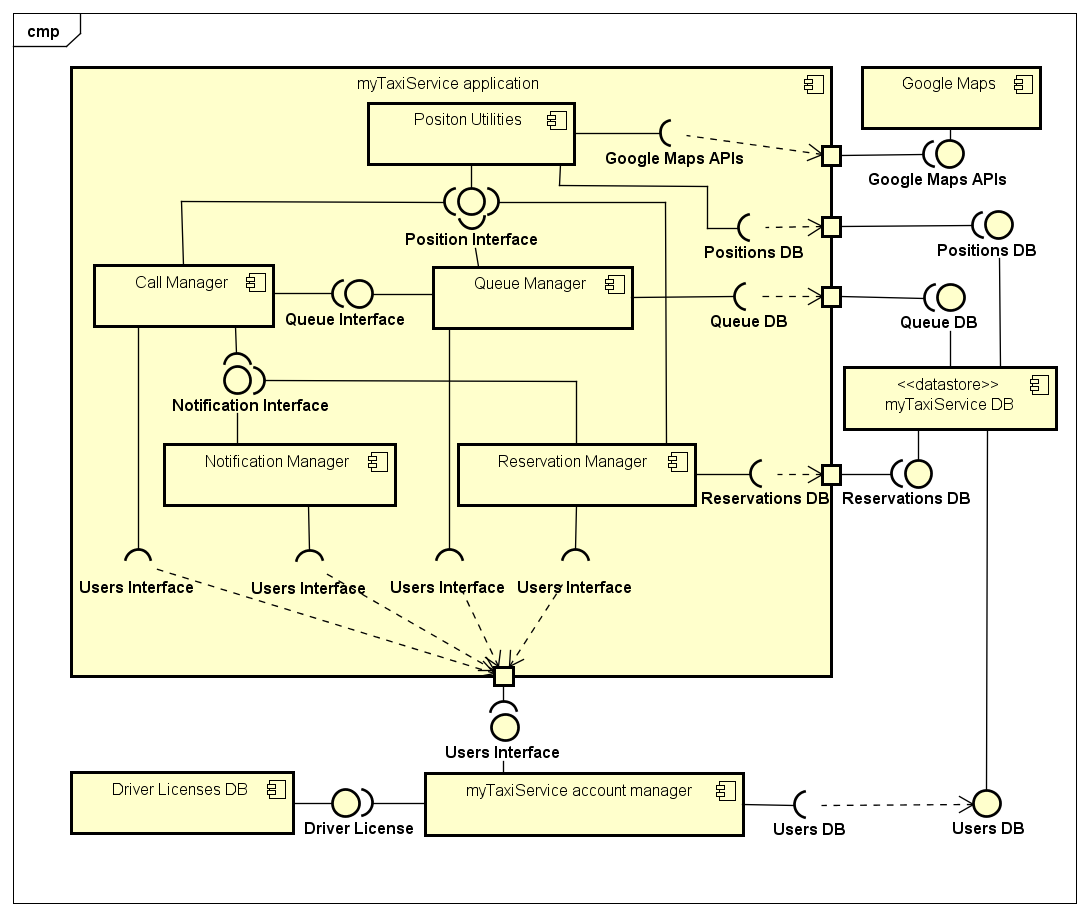
\includegraphics[width=.9\textwidth]{ComponentDiagram}
\centering
\caption{UML Component Diagram}
\label{fig:componentsiagram}
\end{figure}

\subsection{Deployment view}

\vbox{
The following diagram represent the hardware components of the system. For each piece of hardware is also shown what part of software runs on it referring to the components presented in the previous section.
}

\nopagebreak

\begin{figure}[H]
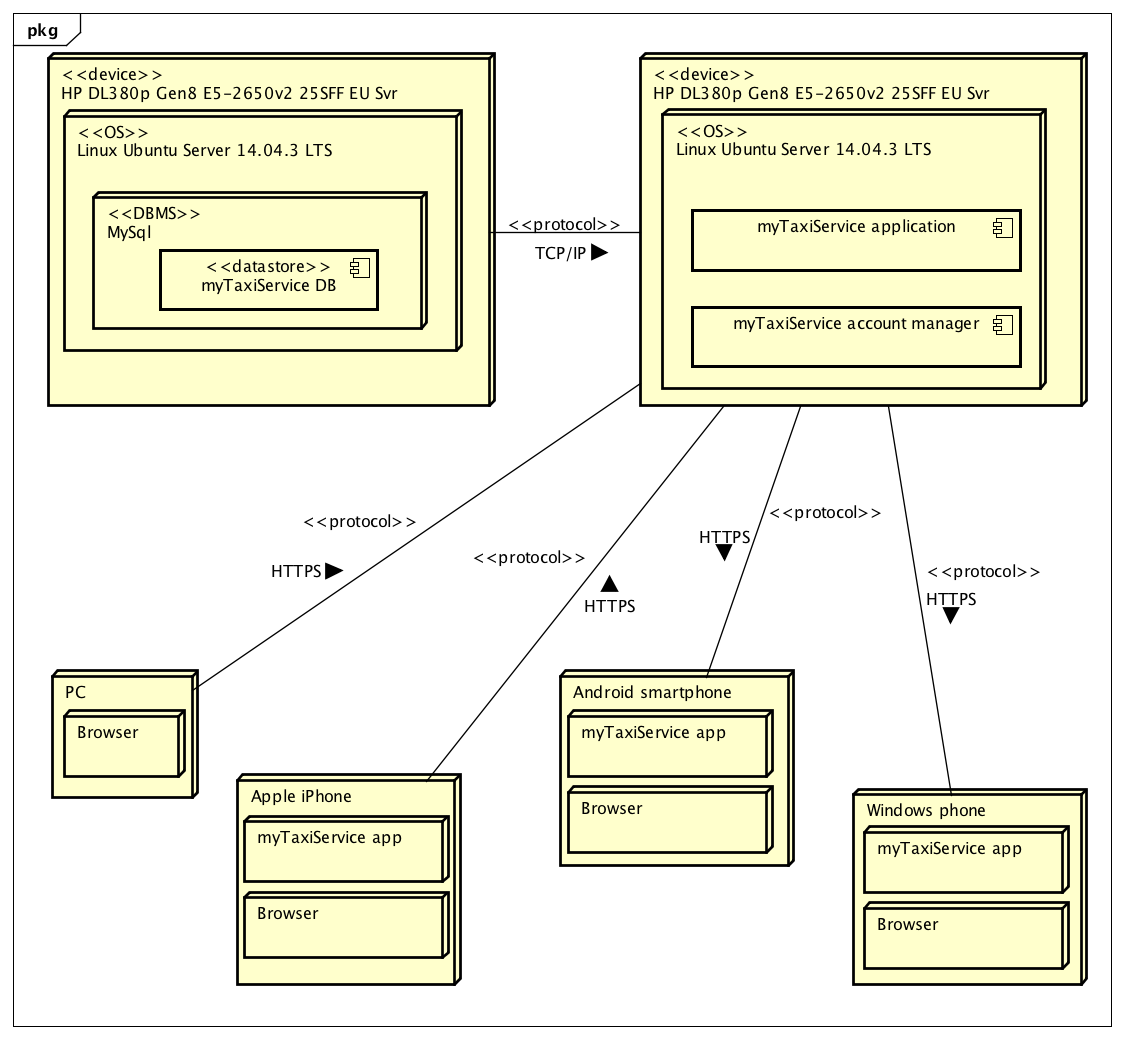
\includegraphics[width=.9\textwidth]{DeploymentDiagram}
\centering
\caption{UML Deployment Diagram}
\label{fig:deploymentsiagram}
\end{figure}

\subsection{Runtime view}

In this section, with some sequence diagrams, are shown the most important interactions between components.

% Sequences Width
\newlength{\sequenceWidth}
\setlength{\sequenceWidth}{\textwidth}

\begin{figure}[H]
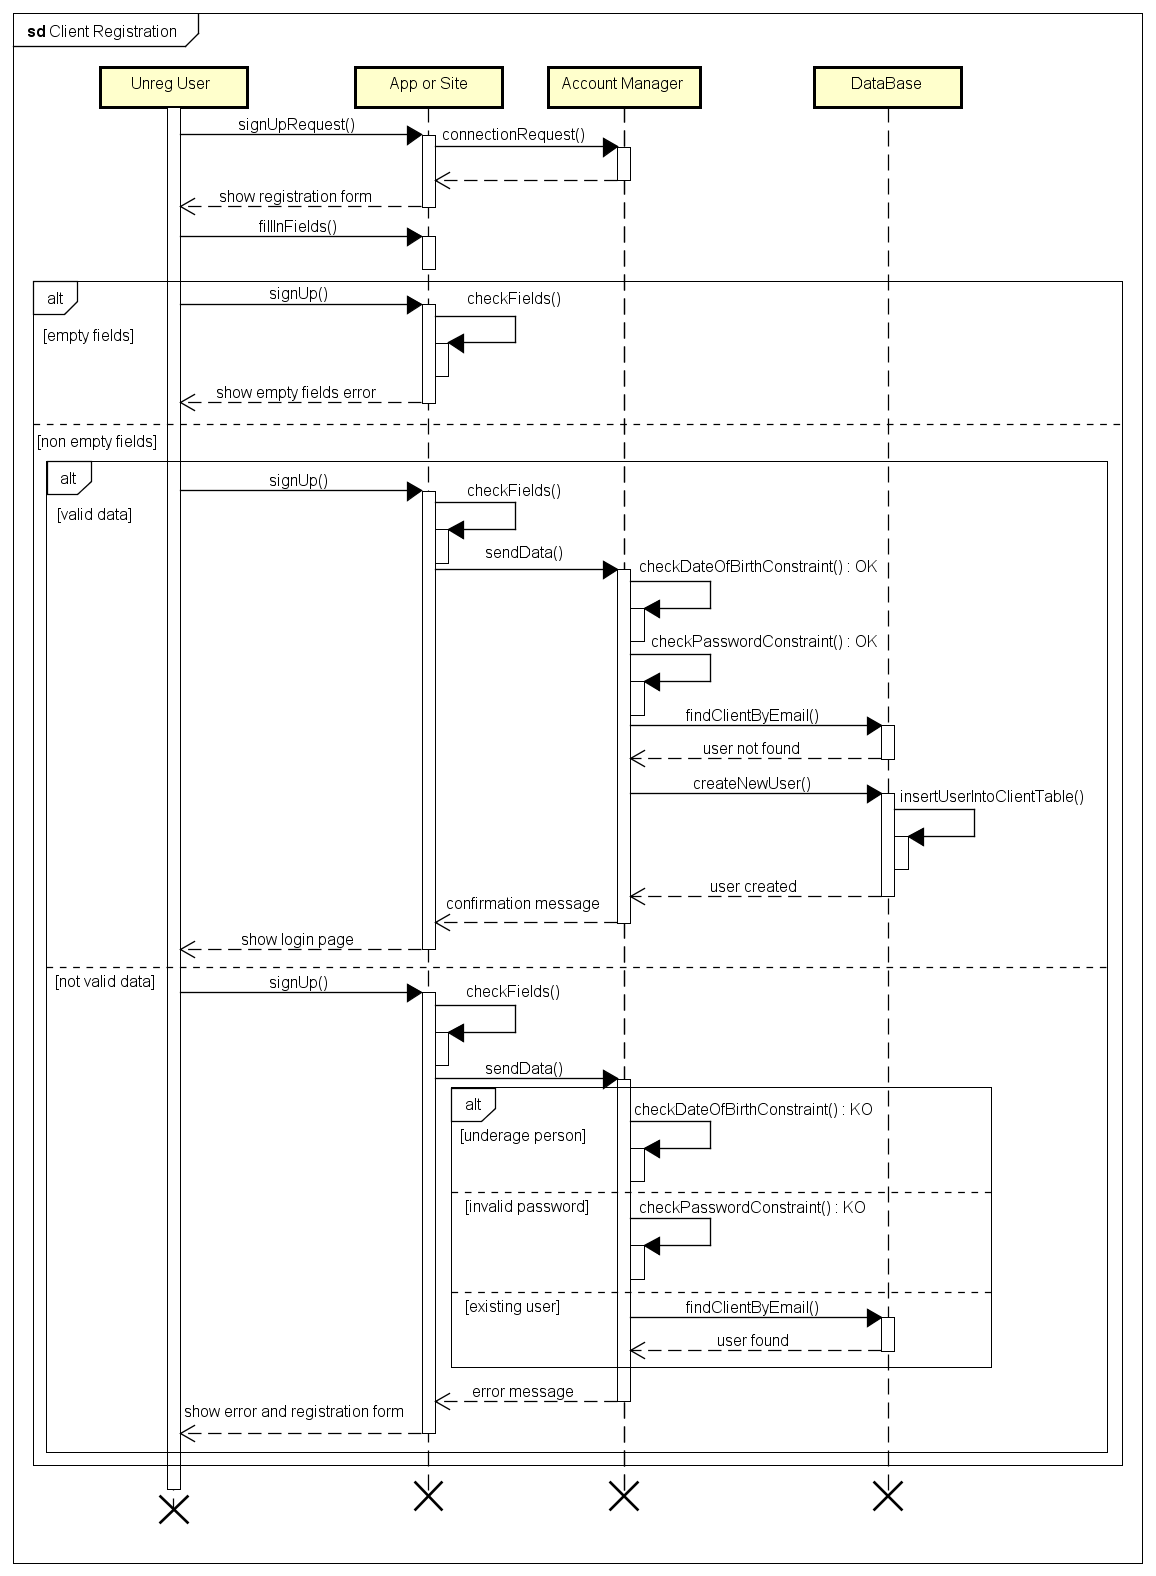
\includegraphics[width=\sequenceWidth]{Sequence-ClientRegistration}
\centering
\caption{Client Registration UML Sequence Diagram}
\label{fig:sequenceclientregistration}
\end{figure}

\begin{figure}[H]
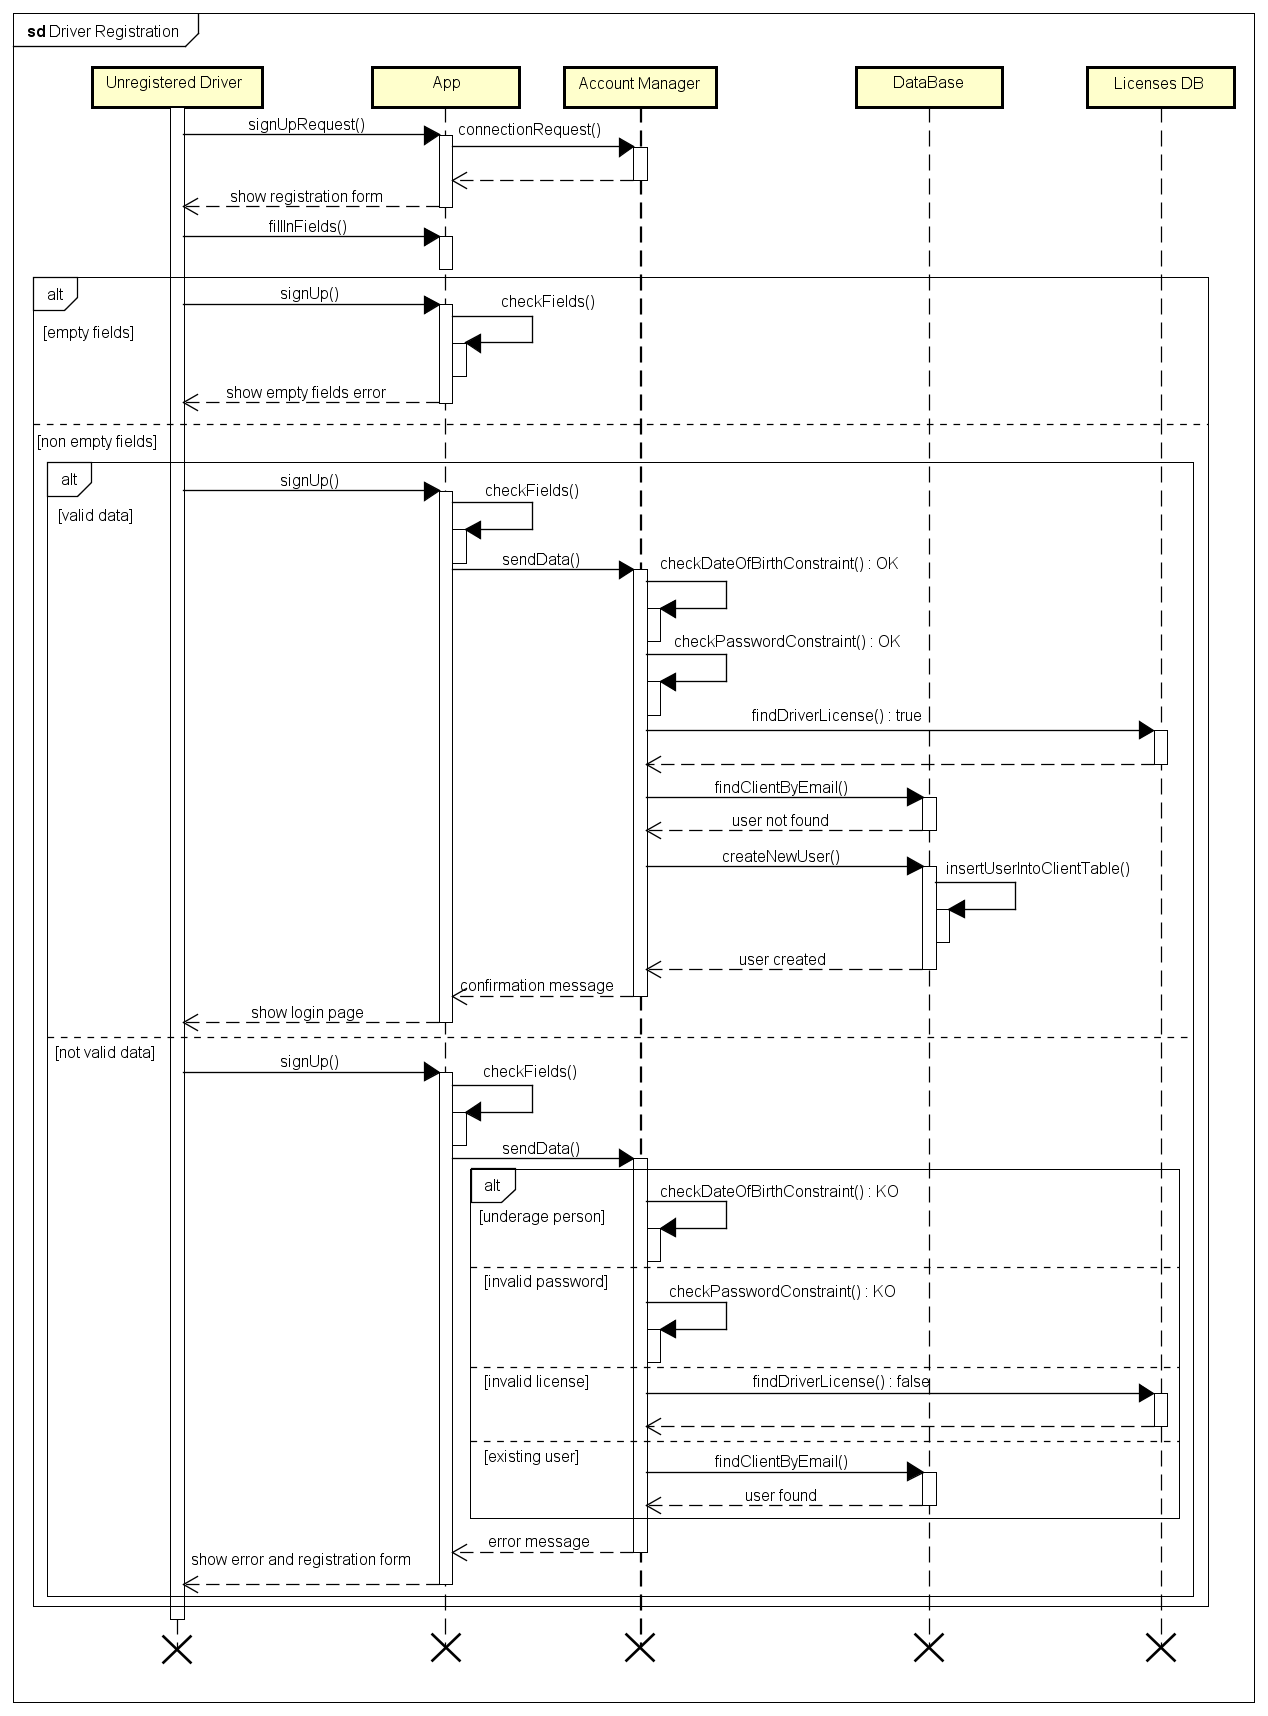
\includegraphics[width=\sequenceWidth]{Sequence-DriverRegistration}
\centering
\caption{Taxi Driver Registration UML Sequence Diagram}
\label{fig:sequencedriverregistration}
\end{figure}

\begin{figure}[H]
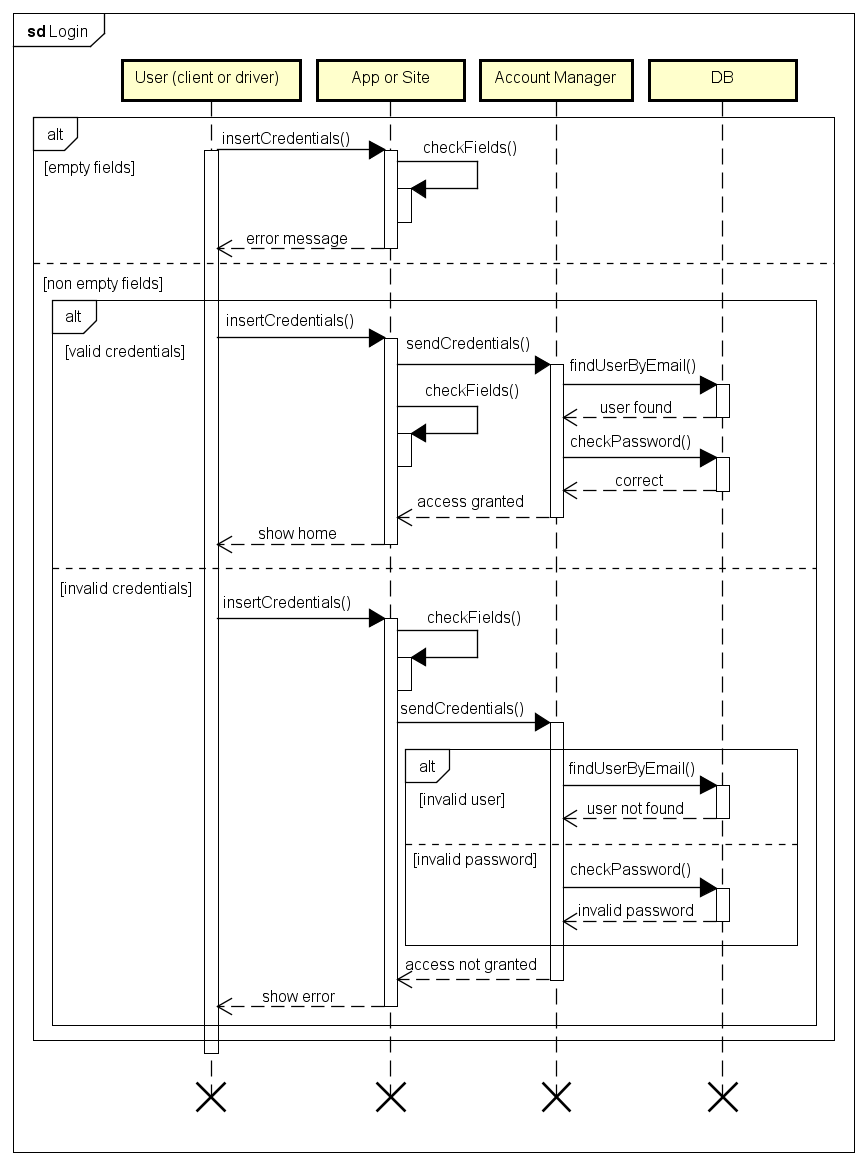
\includegraphics[width=\sequenceWidth]{Sequence-Login}
\centering
\caption{Login UML Sequence Diagram}
\label{fig:sequencelogin}
\end{figure}

\begin{figure}[H]
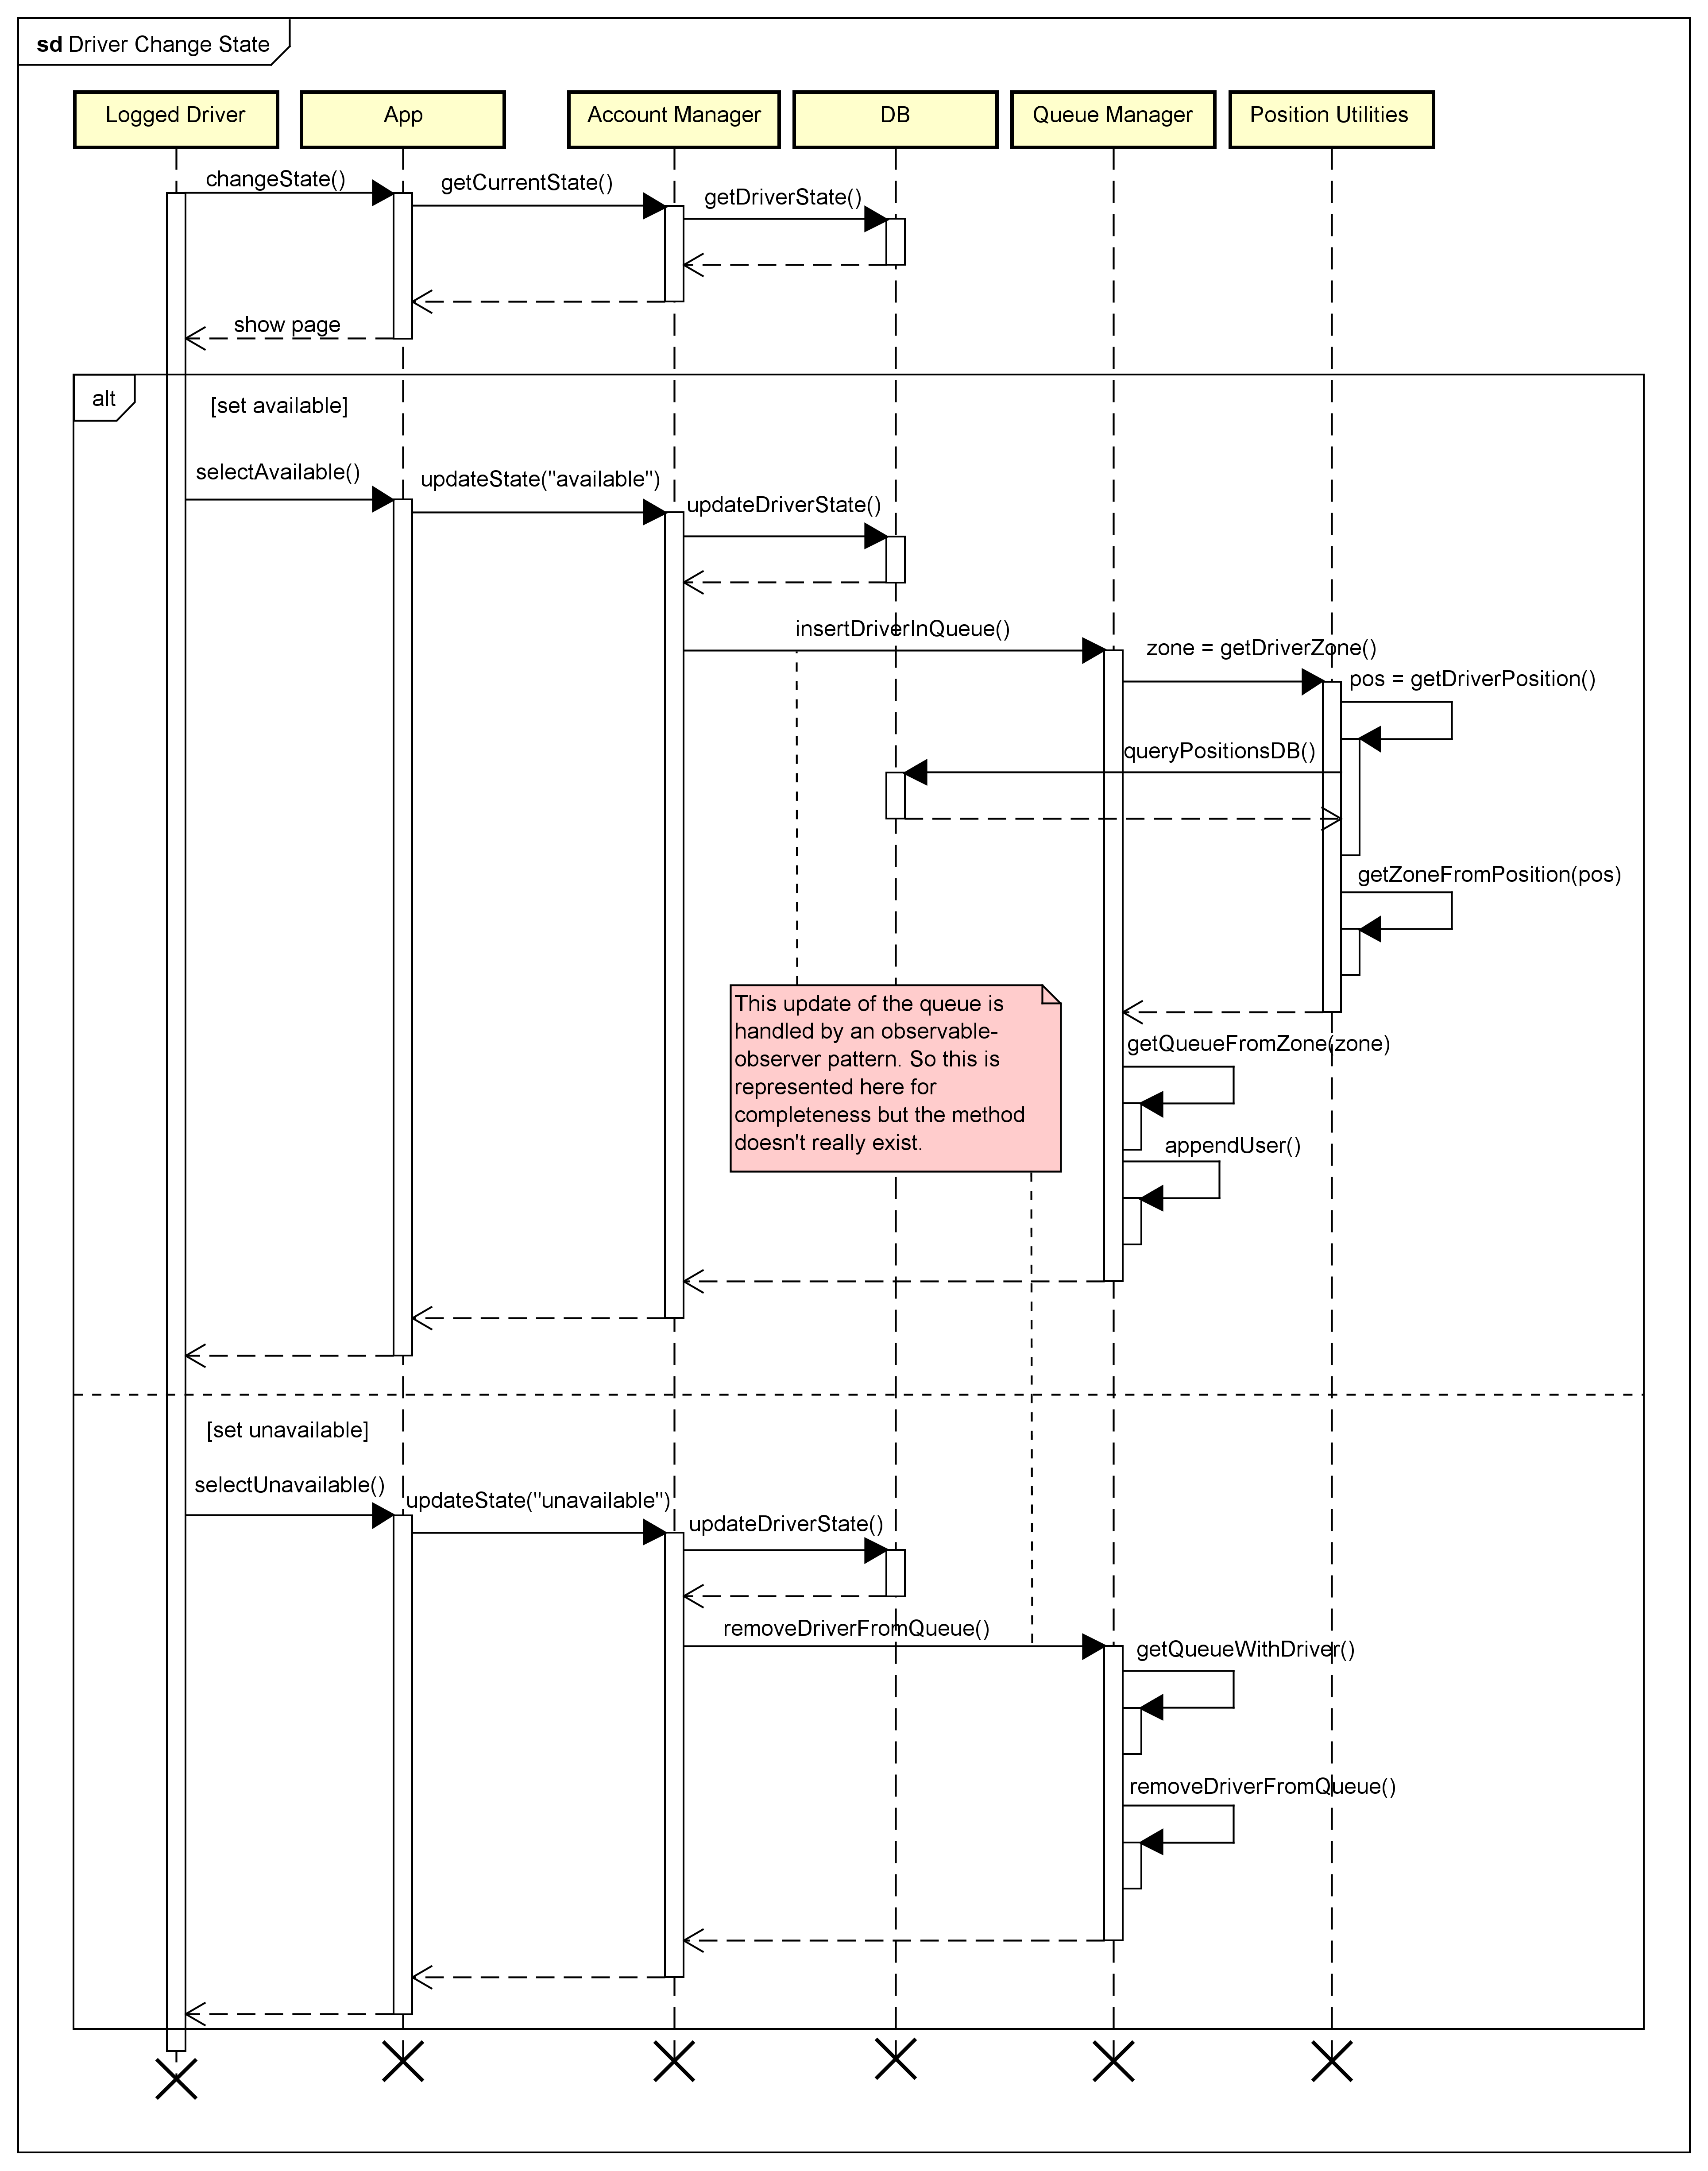
\includegraphics[width=\sequenceWidth]{Sequence-DriverChangeState}
\centering
\caption{Taxi Driver Changes State UML Sequence Diagram}
\label{fig:sequencedriverstate}
\end{figure}

\begin{figure}[H]
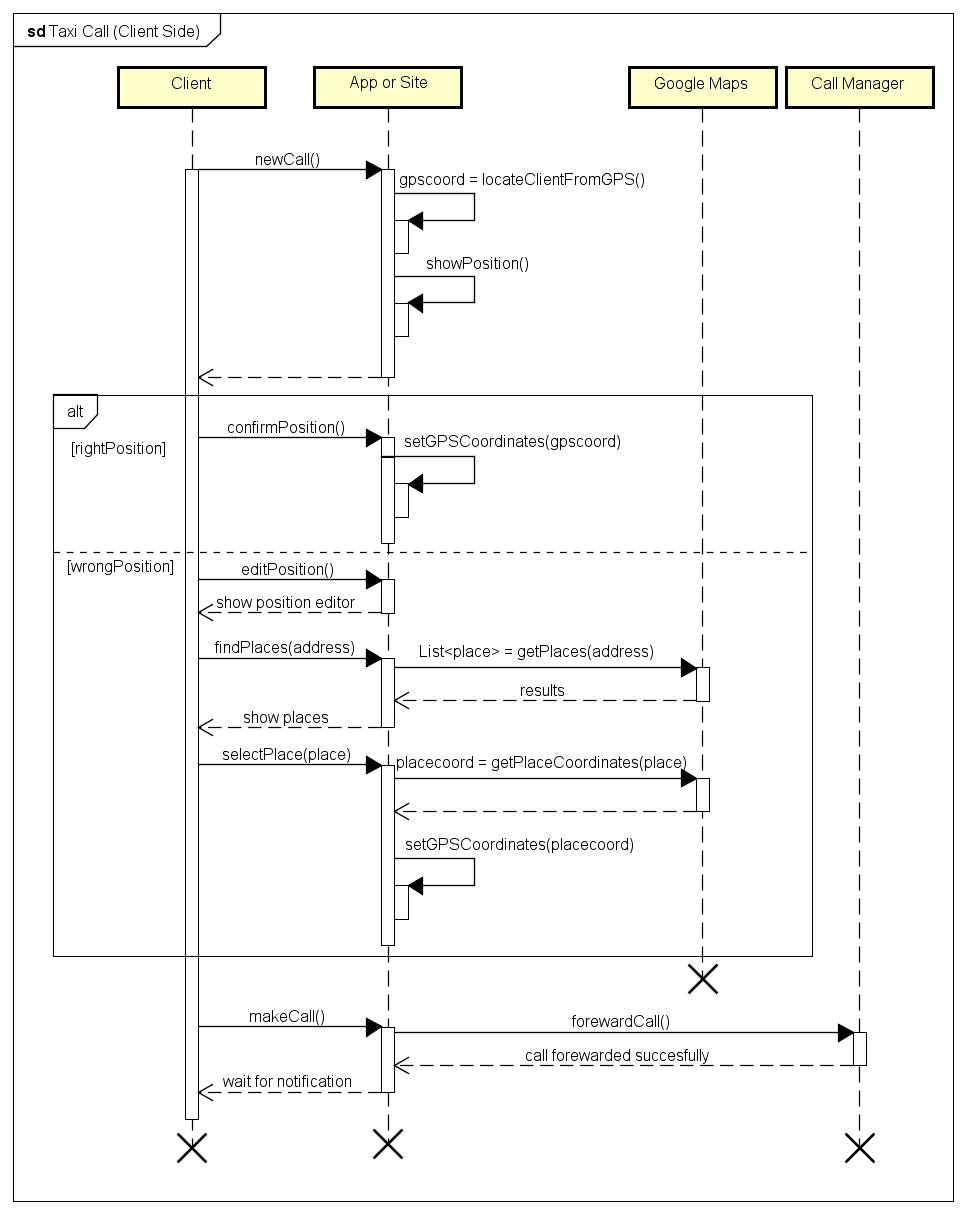
\includegraphics[width=\sequenceWidth]{Sequence-TaxiCallClientSide}
\centering
\caption{Taxi Call Client Side UML Sequence Diagram}
\label{fig:sequencecallclientside}
\end{figure}

\begin{figure}[H]
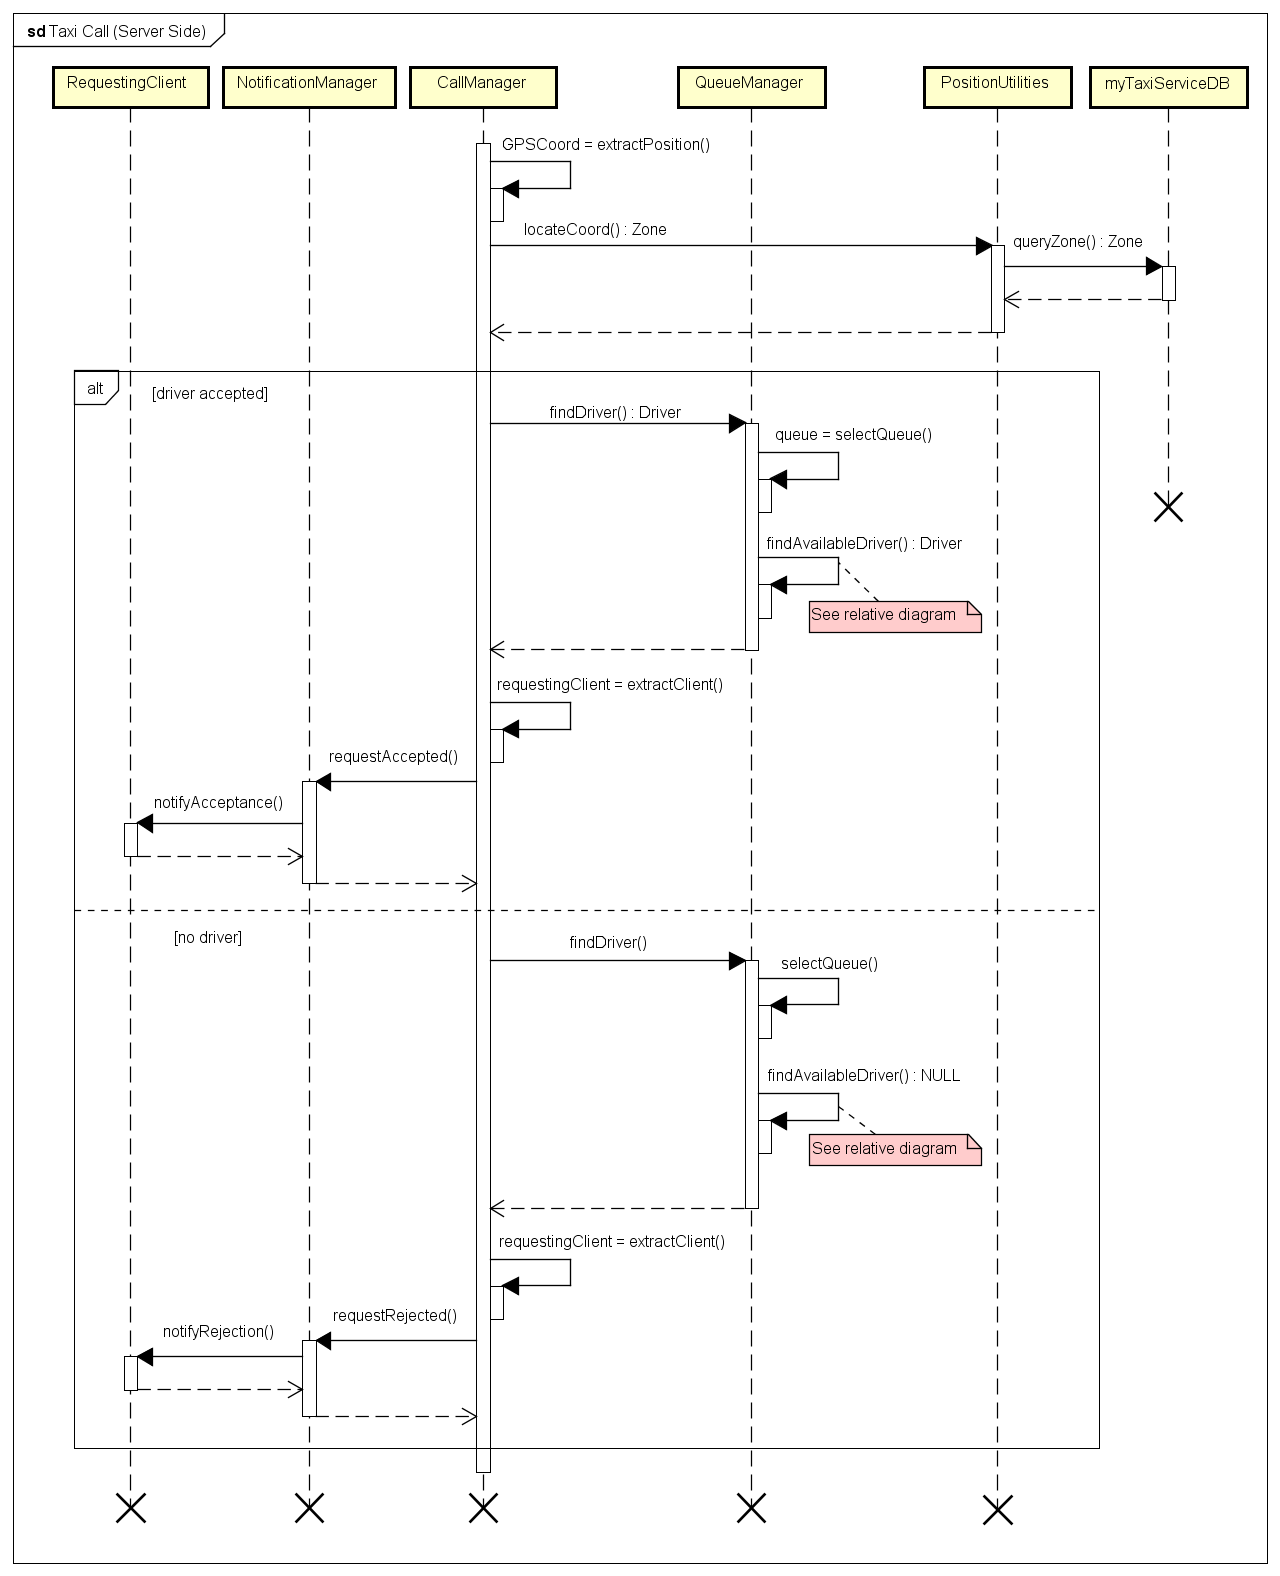
\includegraphics[width=\sequenceWidth]{Sequence-TaxiCallServerSide}
\centering
\caption[Taxi Call Server Side UML Sequence Diagram]{Taxi Call Server Side UML Sequence Diagram: \newline \centering See \autoref{fig:sequencefindavailabledriver} in order to understand what happens in the \emph{findAvailableDriver()} method.}
\label{fig:sequencecallserverside}
\end{figure}

\begin{figure}[H]
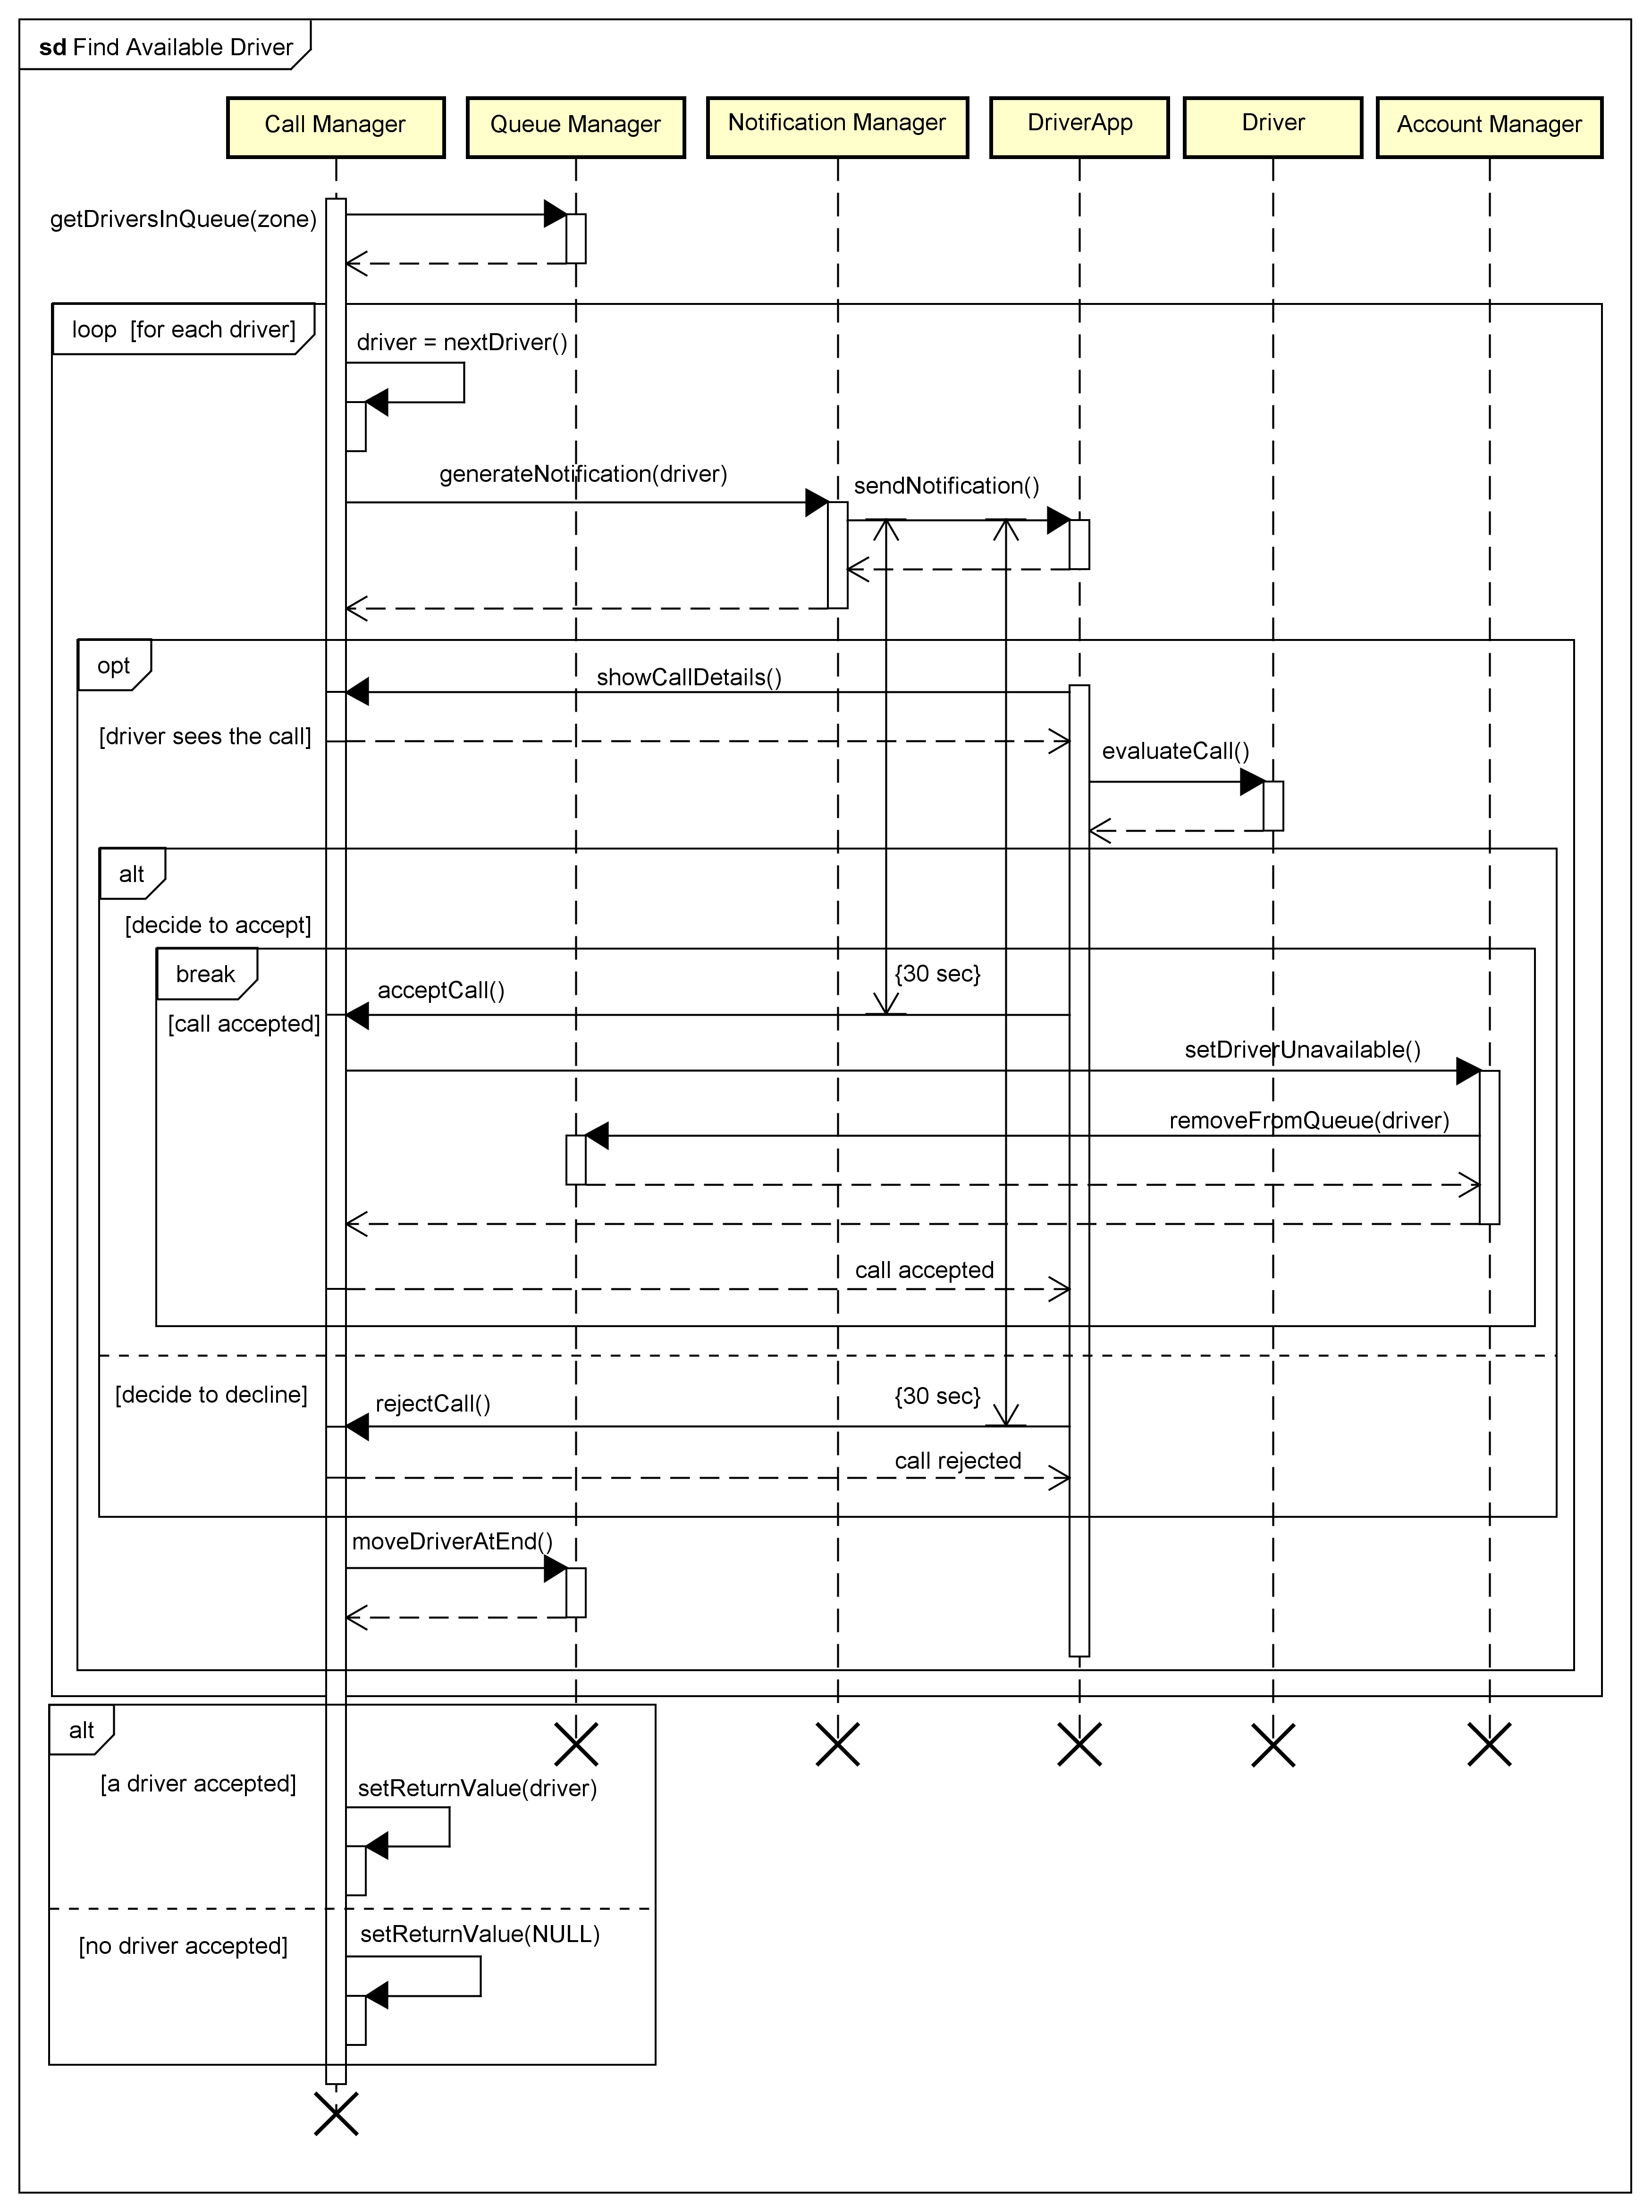
\includegraphics[width=\sequenceWidth]{Sequence-FindAvailableDriver}
\centering
\caption[Find Available Driver UML Sequence Diagram]{Find Available Driver UML Sequence Diagram: \newline
\centering For other details relative to this diagram you can see also \autoref{alg:findavailabledriver}}
\label{fig:sequencefindavailabledriver}
\end{figure}

\begin{figure}[H]
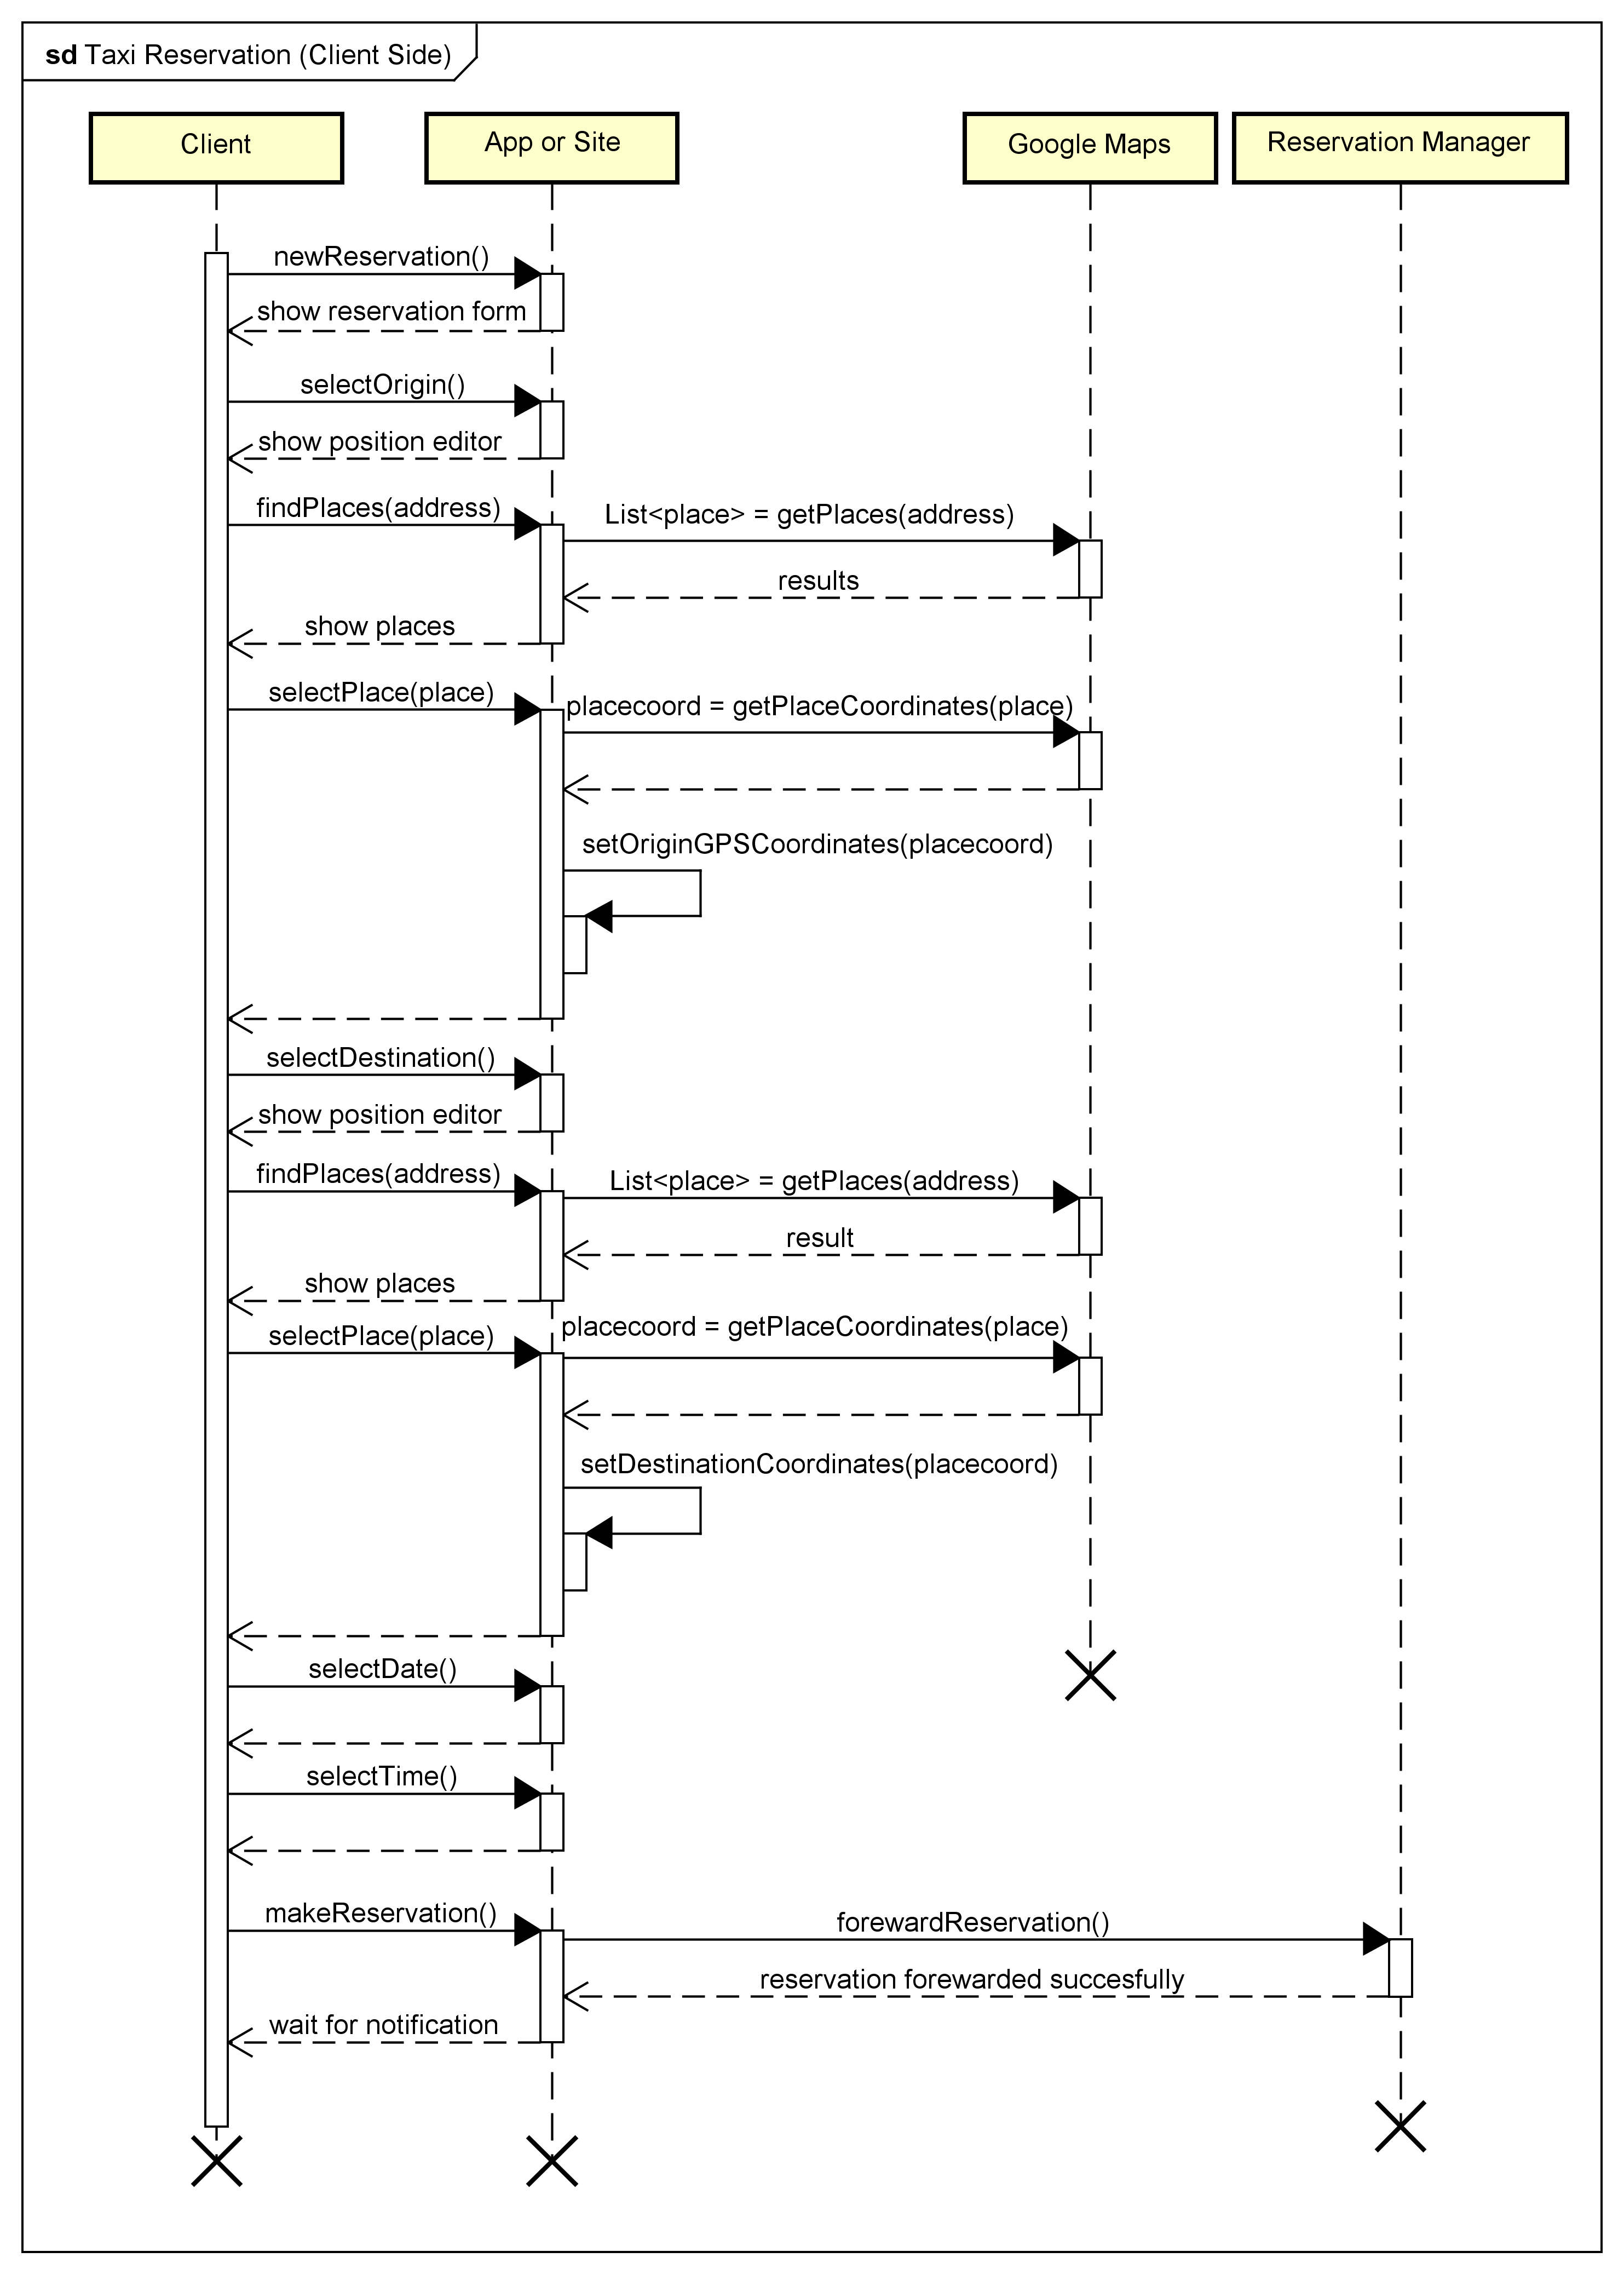
\includegraphics[width=\sequenceWidth]{Sequence-TaxiReservationClientSide}
\centering
\caption{Taxi Reservation Client Side UML Sequence Diagram}
\label{fig:sequencereservationclientside}
\end{figure}

\begin{figure}[H]
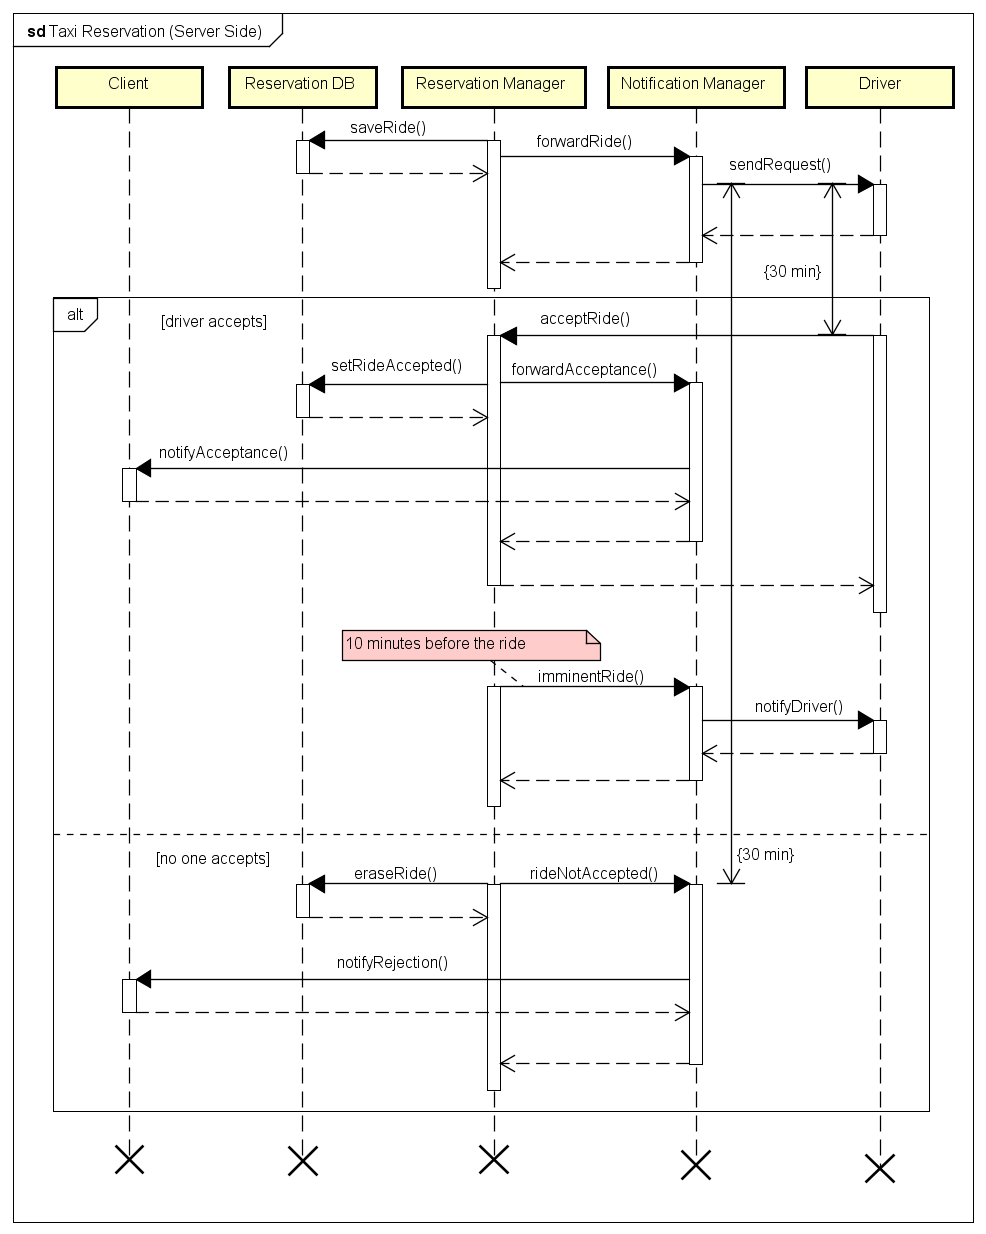
\includegraphics[width=\sequenceWidth]{Sequence-TaxiReservationServerSide}
\centering
\caption{Taxi Reservation Server Side UML Sequence Diagram}
\label{fig:sequencereservationserverside}
\end{figure}

\begin{figure}[H]
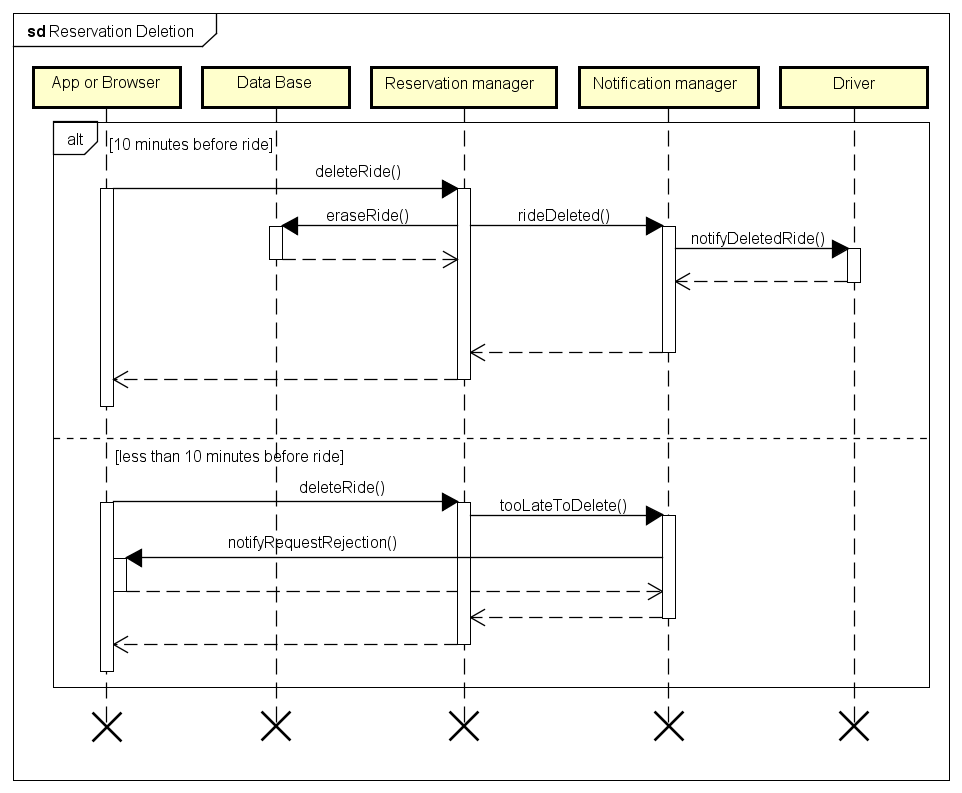
\includegraphics[width=\sequenceWidth]{Sequence-TaxiReservationDeletion}
\centering
\caption{Taxi Reservation Deletion UML Sequence Diagram}
\label{fig:sequencereservationdeletion}
\end{figure}

\subsection{Component Interfaces}

\begin{description}
\item[Data Base:]
\item[Account Manager:] \
\begin{itemize*}
    \item \textit{login(mail, password)}
    \item \textit{registerClient(email, firstName, lastName, telephoneNumber, password)}
    \item \textit{registerDriver(email, firstName, lastName, telephoneNumber, license, password)}
    \item To receive information about an user: \textit{userInfo(email)}
    \item To change a driver state when they are taking a call: \textit{changeDriverState(email, state)}
\end{itemize*}
\item[Call Manager:]\
\begin{itemize*}
    \item To call a taxi: \textit{forwardCall(email, GPSPosition)}
    \item To show the details of a call (should be used by a driver): \textit{showCallDetails(call)}
\end{itemize*}
\item[Queue Manager:]\
\begin{itemize*}
    \item To retrieve the drivers' queue of a certain zone: \textit{driversQueue(zone)}
\end{itemize*}
\item[Reservation Manager:]\
\begin{itemize*}
    \item \textit{newReservation(email, origin, destination, time)}
    \item to show the details of a reservation: \textit{showReservationDetails(reservation)}
\end{itemize*}
\item[Notification Manager:]\
\begin{itemize*}
    \item \textit{sendNotification(list\textless email \textgreater, message)} 
\end{itemize*}
\item[Position Utilities:]\
\begin{itemize*}
    \item to find the zone associated to a given coordinate: \textit{findZone(GPSCoordinate)}
\end{itemize*}
\end{description}

\subsection{Selected Architectural Styles and Patterns}

For this service was selected a \emph{three-tier} architecture: Data, Application Logic and GUI are separated and there are two levels of firewalls in order to keep a high level of security.

In \autoref{fig:architecture} you can see a graphical representation of this architecture.

\nopagebreak

\begin{figure}[H]
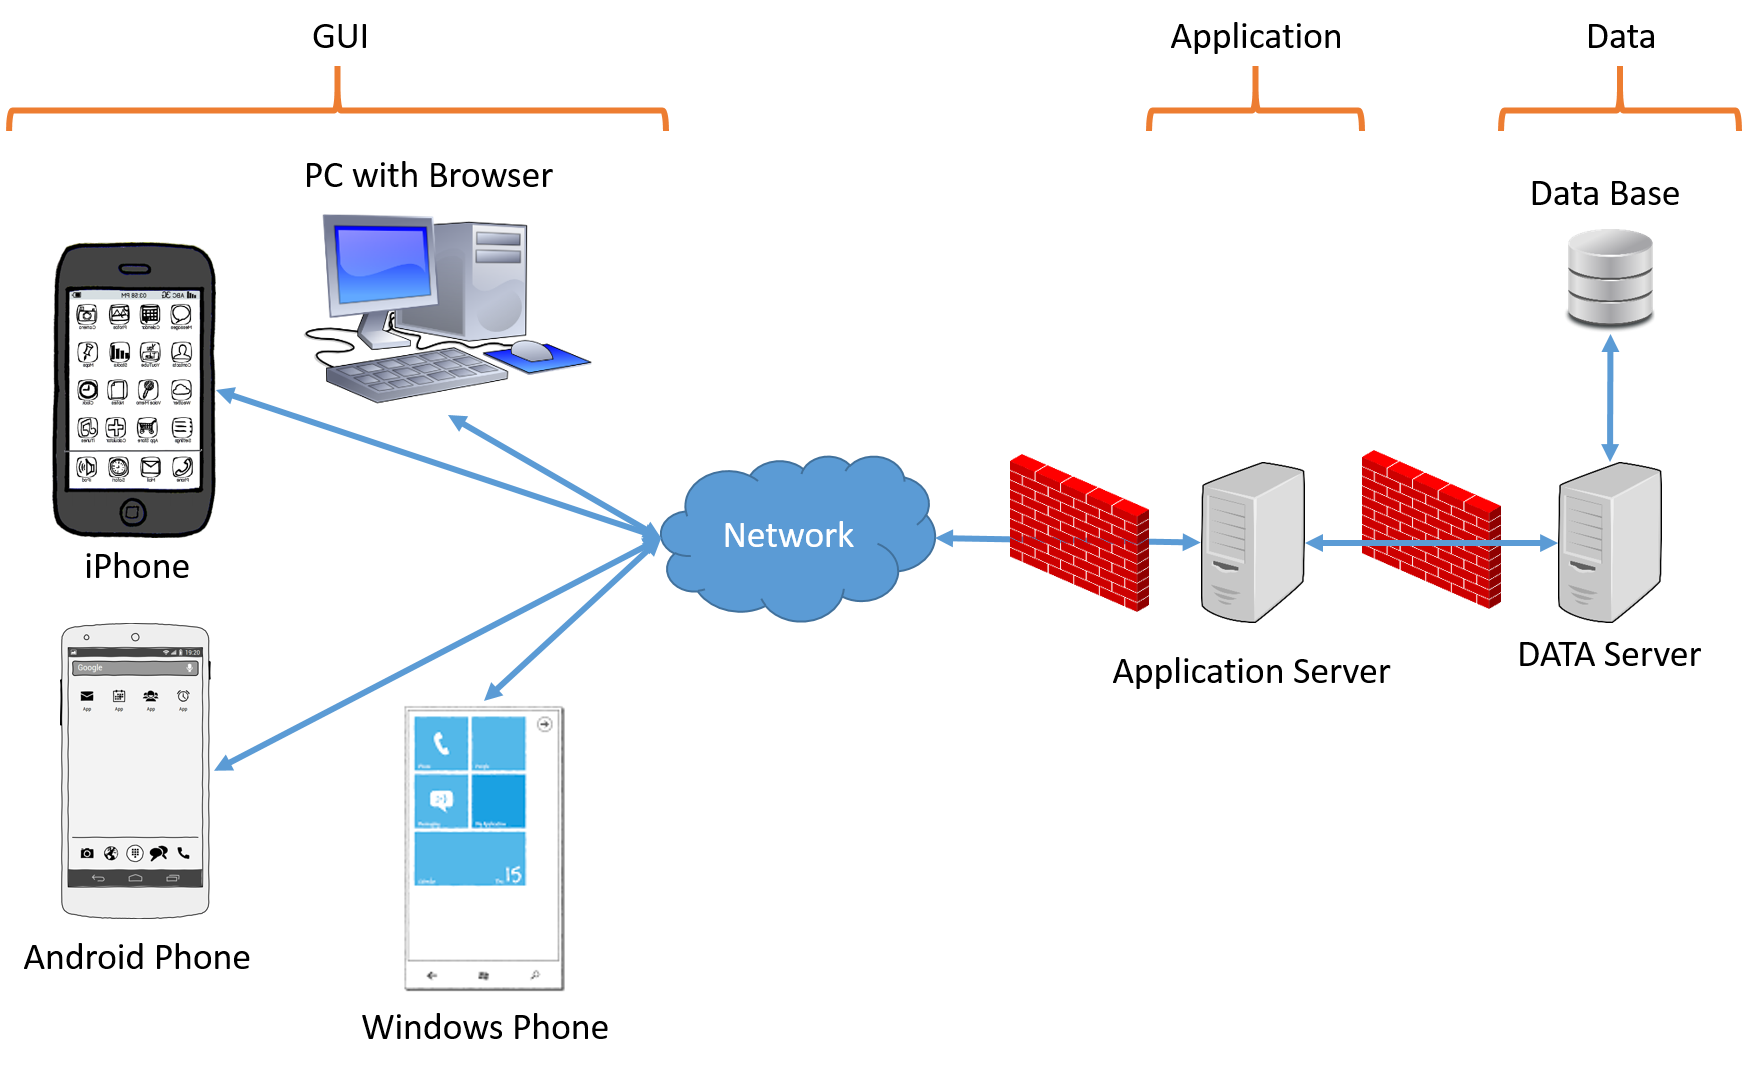
\includegraphics[width=.9\textwidth]{Architecture}
\centering
\caption{Architecture Representation}
\label{fig:architecture}
\end{figure}

About the paradigm we decided to combine two important patterns: 
\begin{itemize*}
\item the \textbf{client-server}
\item the \textbf{publisher-subscriber}
\end{itemize*}

The client server is used for all the communications which are composed by a request, made by the client, and a response, given by the server.

The publisher-subscriber is needed for the notification service.

\begin{figure}[H]
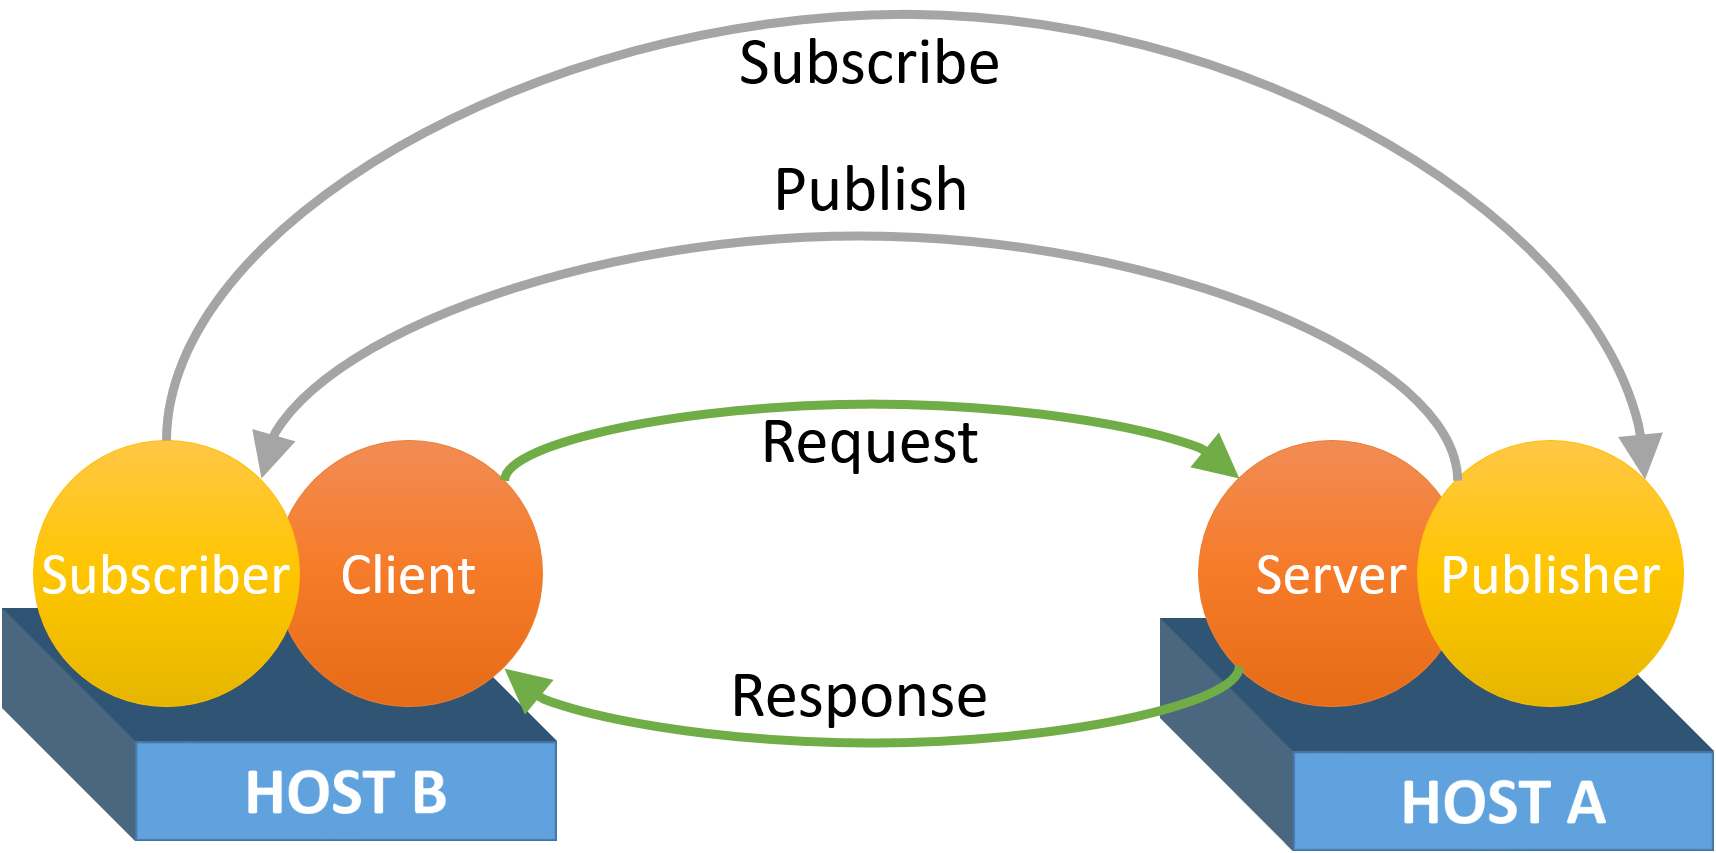
\includegraphics[width=.65\textwidth]{Paradigm}
\centering
\caption{Paradigm Representation}
\label{fig:paradigm}
\end{figure}

\section{Algorithm Design}
\label{sec:sec3}

\emph{myTaxiService} is not a very algorithmic system but there is a little part that is worth describing.
This part is the managing of the queue when a call arrives and is presented in the following algorithm.

\begin{center}
\begin{minipage}{.8\textwidth}
\begin{algorithm}[H]
\caption{Find Available Driver}
\label{alg:findavailabledriver}
\algsetup{indent=2em}
\begin{algorithmic}
    
    \REQUIRE the queue of a zone
    \ENSURE the return value is the driver who accepted the ride or NULL if nobody accepted
    
    \FORALL {drivers in queue (only once)}
        \STATE send a notification to the driver
        \STATE wait for 30 seconds (or less if a response is received)
        \IF {the driver has accepted}
            \STATE remove driver from the queue
            \STATE set driver state as \emph{unavailable}
            \STATE send a notification to the client
            \RETURN current driver
        \ELSIF {the driver has rejected \OR the driver hasn't responded}
            \STATE move the driver from the begin to the end of the queue
        \ENDIF
    \ENDFOR
    \RETURN NULL
\end{algorithmic}
\end{algorithm}
\end{minipage}
\end{center}

\section{User Interface Design}
A complete description of how the user interfaces of our system will look like was already included in our \emph{Requirements and Specification Document} document. You can find it in Section 3.3 \emph{External Interfaces} of the specified document.

\section{Requirements traceability}

\renewcommand{\arraystretch}{1.15}
\def \customTableWidth{12cm}
\newcolumntype{M}{>{\centering\arraybackslash} m{1.15cm} }

\begin{table} [H]
\begin{center}
\begin{tabular}{ |M|M|m{\customTableWidth}|  }
\hline
    \multicolumn{2}{|c|}{\textbf{\textit{Requirement}}}
&   \multicolumn{1}{c|}{\textbf{\textit{Designated system element}}}
\\ 

\hline
\hline

    \multirow{5}{*}{\textbf{G1}} & \textbf{R1} & \multirow{3}{*}{Validation made by the \textit{account manager}}\\
    \cline{2-2} & \textbf{R2}&\\
    \cline{2-2} & \textbf{R3}&\\
    \cline{2-3} & \textbf{R4} & The \textit{account manager} checks if the e-mail address is already inside the \textit{Users DB} \\
    \cline{2-3} & \textbf{R5} & The \textit{account manager} checks if the e-mail address is already inside the \textit{Users DB} and the app or browser shows only the login page and the registration form\\
    
    \hline
    \hline
    
    \multirow{6}*{\textbf{G2}} & \textbf{R1} & \multirow{3}{\customTableWidth}{Validation made by the \textit{account manager}}\\
    \cline{2-2} & \textbf{R2}&\\
    \cline{2-2} & \textbf{R3}&\\
    \cline{2-3} & \textbf{R4} & The \textit{account manager} checks if the driver license is inside the \textit{taxi drivers DB} \\
    \cline{2-3} & \textbf{R5} & The \textit{account manager} checks if the e-mail address is already inside the \textit{Users DB}\\
    \cline{2-3} & \textbf{R6} & The \textit{account manager} checks if the e-mail address is already inside the \textit{Users DB} and the app or browser shows only the login page and the registration form\\
    
    \hline
    \hline
    
    \multirow{4}*{\textbf{G3}} & \textbf{R1} & \multirow{4}{\customTableWidth}{Validation made by the \textit{account manager}}\\
    \cline{2-2} & \textbf{R2}&\\
    \cline{2-2} & \textbf{R3}&\\
    \cline{2-2} & \textbf{R4}&\\
    
    \hline
    \hline
    
    \multirow{3}*{\textbf{G4}} & \textbf{R1} & \multirow{3}{\customTableWidth}{Validation made by the \textit{account manager}}\\
    \cline{2-2} & \textbf{R2}&\\
    \cline{2-2} & \textbf{R3}&\\
    
    \hline
    \hline
    
    \multirow{4}*{\textbf{G5}} & \textbf{R1} & Validation made by the \textit{account manager}\\
    \cline{2-3} & \textbf{R2}&\multirow{3}{\customTableWidth}{\textit{App} or \textit{browser} running on a device with enabled GPS and connected to the internet}\\
    \cline{2-2} & \textbf{R3}&\\
    \cline{2-2} & \textbf{R4}&\\

    \hline
    \hline
    
    \multirow{2}*{\textbf{G6}} & \textbf{R1} & Validation made by the \textit{account manager}\\
    \cline{2-3} & \textbf{R2} & {The \textit{Queue manager} receives a positive answer from one of the taxi}\\
    
    \hline
    \hline
    
    \multirow{2}*{\textbf{G7}} & \textbf{R1} & Validation made by the \textit{account manager}\\
    \cline{2-3} & \textbf{R2} & {The \textit{Queue manager} receives a positive answer from one of the taxi}\\
    
    \hline
    \hline
    
    \multirow{2}*{\textbf{G8}} & \textbf{R1} & Validation made by the \textit{account manager}\\
    \cline{2-3} & \textbf{R2} & {Time out for the \textit{Queue manager} which was waiting for a positive answer}\\
    
    \hline
    \hline
    
    \multirow{3}*{\textbf{G9}} & \textbf{R1} & Validation made by the \textit{account manager}\\
    \cline{2-3} & \textbf{R2} & \textit{Driver app} running on their smartphone\\
    \cline{2-3} & \textbf{R3} & \textit{Position utilities} stored driver position in the \textit{positions' DB}\\
    
    \hline
    \hline
    
    \textbf{G10} & \textbf{R1} & Validation made by the \textit{account manager}\\
    
    \hline
    
\end{tabular}
\end{center}
\label{table:requirementsTraceabilityPt1}
\caption{Requirements traceability part 1}
\end{table}

\begin{table} [H]
\begin{center}
\begin{tabular}{ |M|M|m{\customTableWidth}|  }
\hline
    \multicolumn{2}{|c|}{\textbf{\textit{Requirement}}}
&   \multicolumn{1}{c|}{\textbf{\textit{Designated system element}}}
\\ 

    \hline
    \hline

    \multirow{4}*{\textbf{G11}} & \textbf{R1} & Validation made by the \textit{account manager}\\
    \cline{2-3} & \textbf{R2} & \textit{Account manager} checks the \textit{users DB}\\
    \cline{2-3} & \textbf{R3} & \textit{Queue manager} works with the \textit{position utilities} to select the right queue in the \textit{queue DB}\\
    \cline{2-3} & \textbf{R4} & \textit{Notification manager} sends a notification to the {driver app}\\

    \hline
    \hline

    \multirow{4}*{\textbf{G12}} & \textbf{R1} & Validation made by the \textit{account manager}\\
    \cline{2-3} & \textbf{R2} & \textit{Account manager} checks the \textit{users DB}\\
    \cline{2-3} & \textbf{R3} & \textit{Queue manager} updates driver's state working with the \textit{account manager} \\
    \cline{2-3} & \textbf{R3} & \textit{Queue manager} works with the \textit{position utilities} to select the right queue in the \textit{queue DB}\\
    
    \hline
    \hline

    \multirow{4}*{\textbf{G13}} & \textbf{R1} & Zones are saved in the \textit{myTaxiServiceDB}\\
    \cline{2-3} & \textbf{R2} & \multirow{3}{\customTableWidth}{\textit{Position utilities} locate drivers in a zone, \textit{queue manager} updates the zone's queue, the \textit{account manager} checks driver's state in the \textit{users DB}}\\
    \cline{2-2} & \textbf{R3} &\\
    \cline{2-2} & \textbf{R4} &\\
    
    \hline
    \hline
    
    \multirow{11}*{\textbf{G14}} & \textbf{R1} & The \textit{call manager receives the taxi call}\\
    \cline{2-3} & \textbf{R2} & \textit{Queue manager} works with the \textit{position utilities} to locate drivers in the zone, then the \textit{notification manager} sends the request to the first driver in the queue\\
    \cline{2-3} & \textbf{R3} & The \textit{queue manager} receives a positive answer, then the \textit{notification manager} sends a notification to the client\\
    \cline{2-3} & \textbf{R4} & The \textit{queue manager} wait for 30 seconds an answer from the first client then selects the second driver and asks to the \textit{notification manager} to send a message to them\\
    \cline{2-3} & \textbf{R5} & The \textit{queue manager} updates the \textit{queue DB} positioning the driver at the bottom of their zone's queue \\

    \hline
    \hline
    
    \multirow{3}*{\textbf{G15}} & \textbf{R1} & Validation made by the \textit{account manager}\\
    \cline{2-3} & \textbf{R2} & \multirow{2}{\customTableWidth}{Validation made by the \textit{reservation manager}}\\
    \cline{2-2} & \textbf{R3} &\\

    \hline
    \hline
    
    \multirow{7}*{\textbf{G16}} & \textbf{R1} & The \textit{reservation manager} receives the client's reservation\\
    \cline{2-3} & \textbf{R2} & The \textit{reservation manager} retrieves the driver's accounts from the \textit{account manager}, then asks the \textit{notification manager} to send the reservation details\\
    \cline{2-3} & \textbf{R3} & \multirow{2}{\customTableWidth}{The \textit{reservation manager} waits an answer for 30 minutes, then it interrupts the reservation process}\\
    \cline{2-2} & \textbf{R4} &\\
    \cline{2-3} & \textbf{R5} & If the \textit{reservation manager} receives a confirmation it asks the \textit{notification manager} to notify the client\\
    \cline{2-3} & \textbf{R6} & The \textit{reservation manager} asks the \textit{notification manager} to notify the client of the rejection of the reservation if 30 minutes have passed and no driver answered positively\\
    \cline{2-3} & \textbf{R7} & The \textit{reservation manager} asks the \textit{notification manager} to notify the drivers 10 minutes before the time of the reservation they accepted\\

    \hline
    \hline

    \textbf{G17} & \textbf{R1} & The \textit{account manager} updates the position and the state of the driver's in the \textit{users DB}\\
    
    \hline


        

\end{tabular}
\end{center}
\label{table:requirementsTraceabilityPt2}
\caption{Requirements traceability part 2}
\end{table}

\section{References}
\todo{?!?!?!?}

\section{Appendix}

\subsection{Software and Tools used}

\begin{description}
\item[ShareLatex:] This web application was used to redact this document in a collaborative way. 
\newline (\url{https://it.sharelatex.com/})
\item[Astah Professional:] This desktop application was used to create all the others UML Diagrams.
\newline (\url{http://astah.net/})
\end{description}

\subsection{Hours of Work}
We spent approximately the following amount of hours to redact this document:
\todo{Add hours of work}
\begin{description}
\item[Riva Luca:] 
\item[Strada Jacopo:] 
\end{description}


\end{document}
